\documentclass[10pt,article]{IEEEtran}

\usepackage{hyperref}
\usepackage{graphicx}	% For figure environment
\usepackage{enumitem}
\usepackage{lipsum}
\usepackage{booktabs}
\usepackage{tabularx}
\usepackage{adjustbox}
\usepackage[compact]{titlesec}
\usepackage{placeins}

\begin{document}
\title{ML Project 1: spot the Higgs boson}

\author{
  Manuel Leone, Gabriele Macchi, Marco Vicentini\\
  \textit{Department of Computer Science, EPFL Lausanne, Switzerland}
}

\maketitle

\begin{abstract}
Machine Learning techniques are becoming increasingly popular nowadays and they are used in several and different fields of science.  These are useful when we deal with complex and high dimensional data sets which, sometimes, represented output of scientific experiments. Thanks to this project we are trying to implement some of these tools in order to work on a problem of binary classification on a data-set which come directly from CERN.
\end{abstract}

\section{Introduction}

The aim of this project is to find the best method to distinguish signals of the High Boson from the background noise thanks to binary classification, we did this by using machine learning methods. We used the CERN’s dataset which summarizes collision experiments. The dataset includes 250.000 categorized events with 30 features for each column. The huge amount of data made us face the problem of selection of features needed and how to approach null values. The data processing is a fundamental step of the project, followed by machine learning methods implementations. We start with the implementation of basic algorithm as Linear Regression, Ridge Regression and Logistic Regression. Implementation and discussion of these algorithms are in Sections~\ref{subsec:model-impl} and ~\ref{subsec:model-proc}.

\section{Models and methods}
\label{sec:models-methods}

Implementing good machine learning methods requires skills in the fields of data analysis and algorithm design. Understanding the story behind the data is fundamental to choose the right direction in the following implementations. On the other hand, the broad panorama of ML algorithms in literature provides several possible implementations, able to change dramatically the performance of the algorithms. Our analysis will develop in depth inside this two aspects.
Before to getting inside the developing process, the reader is advised that the preliminary step performed is a \textbf{dataset division}. Indeed, in order to have a idea of the  goodness of fit and to compare the methods, the algorithms were trained on 80\% of the available dataset and
tested on the remaining 20\%.

\subsection{Basic ML implementations}
\label{subsec:model-impl}
The implementation of the base methods consists of six well known Machine Learning algorithm such as Gradient Descend, Stochastic Gradient Descend, Least Squares, Ridge Regression, Logistic Regression and Regularized Logistic Regression. The null values of the dataset were initially filled with the median of the column. Firstly, the computation concerned the entire dataset. In the table below different hyperparameters and results of the methods are shown. The accuracy achieved is computed on \textbf{our test set}. These results were not satisfactory, so we decided to move on with data processing, as described in the next section.

\begin{table}[h!]
\resizebox{\columnwidth}{!}{%
\centering
\begin{tabular}{|l|l|l|l|l|l|} 
\cline{2-5}
\multicolumn{1}{l|}{}    & \multicolumn{4}{l|}{Hyperparameters Used} & \multicolumn{1}{l}{}  \\ 
\hline
Methods                  & $\lambda$ & $\gamma$ & Degree & Max Iter      & Acc. \\ 
\hline
Gradient Descent         & /      & $10^{-6}$ &   1     &   2000         &  0.718   \\ 
\cline{1-1}
Stochastic GD            & /      & $10^{-7}$ & 1      & 1000         & 0.704    \\ 
\cline{1-1}
Least Squares            & /      &  /      & 1      & /              & 0.741   \\ 
\cline{1-1}
Ridge Regression         & $10^{-8}$ &  /      & 6      & /              &   0.766   \\ 
\cline{1-1}
Logistic Regression      & /      &  $10^{-10}$      & 1      & 10000           &   0.735   \\ 
\cline{1-1}
Reg. Logistic Regression &  $10^{-8}$    &   $10^{-10}$      & 1      & 10000           &            0.735           \\
\hline
\end{tabular}%
}
  \caption{Accuracies of the six algorithms without feature processing}
  \label{tab:firstresults}
\vspace{-0.5cm}
\end{table}

\subsection{Dataset analysis and preprocessing}

% \begin{figure}[tbp]
%   \centering
%   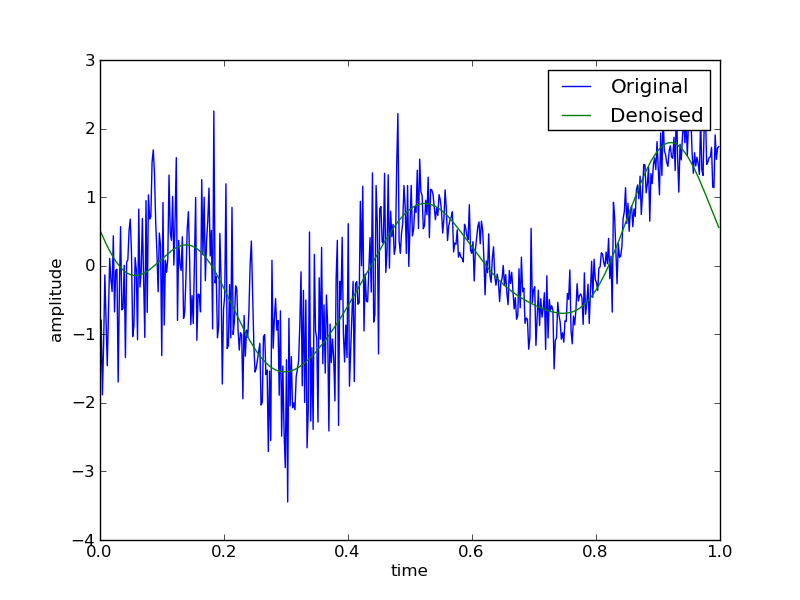
\includegraphics[width=\columnwidth]{denoised_signal_1d}
%   \caption{Signal compression and denoising using the Fourier basis.}
%   \vspace{-3mm}
%   \label{fig:denoise-fourier}
% \end{figure}
% \begin{figure}[htbp]
%   \centering
%   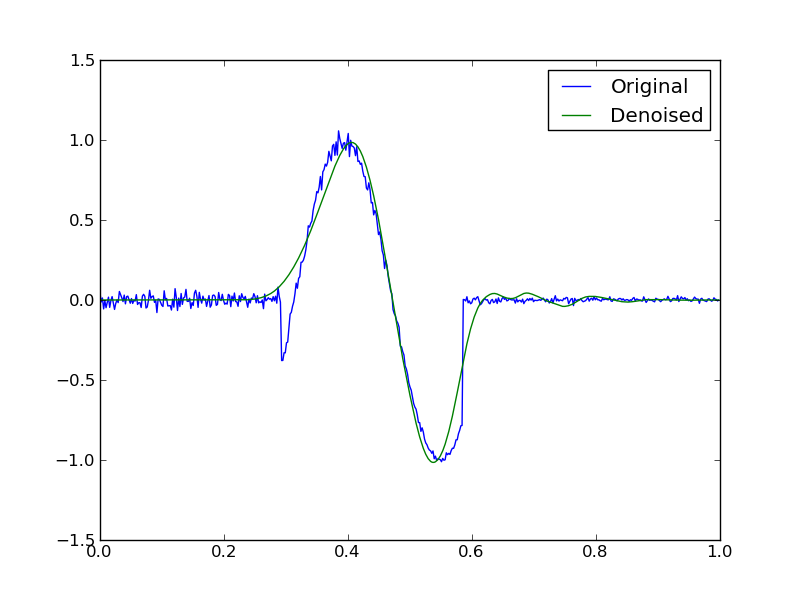
\includegraphics[width=\columnwidth]{local_wdenoised_1d}
%   \vspace{-3mm}
%   \caption{Signal compression and denoising using the Daubechies wavelet basis.}
%   \label{fig:denoise-wavelet}
% \end{figure}

% Use examples and illustrations to clarify ideas and results. For
% example, by comparing Figure~\ref{fig:denoise-fourier} and
% Figure~\ref{fig:denoise-wavelet}, we can see the two different
% situations where Fourier and wavelet basis perform well. 
The analysis of the dataset has been performed in different steps and each of them led to gradually improve the methods performances. The examinations we carried out are the following:
\subsubsection{NaN analysis} The official documentation \cite{higghsdoc} reports the dataset variables as primitive (\texttt{PRI\_}), raw quantities directly measured from the collisions detector, or derived (\texttt{DER\_}), which are computed by the ATLAS physicist using the primitives. This information is useful to understand the physics means behind another fundamental property: the dataset presents many -999.0 as placeholders for missing values. So, our first aim was to understand how we could impute these \textit{NaN}.\\
The analysis of the documentation shows a strict correlation between \textit{NaN} and the \texttt{PRI\_jet\_num} quantity. The jets are, from our understanding of the physic background, the sub particles produced in a collision. The main point to understand here is that some quantities are intentionally undefined because impossible to compute or no-sense with a number of jet equal to 0 or 1. With this cardinal concept in the head, we proceeded to a dataset categorization in four different subset based on the \texttt{PRI\_jet\_num}. As a result, we produced only columns totally full or totally empty from \textit{NaN} values, with the only exception of the \texttt{DER\_mass\_MMC} one.\\
At this point, we dropped all the columns taotally filled with \textit{NaN} values. For the remaining missing elements we tried to use another time classical imputation methods such are using mean or average of the other values in the column. But this procedures never led us to a drastic gain in performance. Skilled by the experience of the previous division, we decided to carry out a second split based on \textit{NaN} remainings in \texttt{DER\_mass\_MMC}, producing a total of eight subset, totally cleaned from all missing values.
\subsubsection{Correlation analysis} To better analyze each of the features we move further to plot the scatter matrix between all of them in all the subsets, in order to understand which of them have an high correlation. We discovered that at this point of the preprocessing pipeline some columns had the same values and a correlation of 1.00. We hypothesize that this features have the same physical meaning when considered only in the subset. To simplify our model and improve the prediction we decide do delete one of the two features.
\subsubsection{Skewness removal} The scatter plot matrix visualization pointed out the presence of many right-skewness distributions features. We applied cube root transformation to this columns to transform them into centered distributions.
\subsubsection{Adding 1s column and standardization} The last steps of the main preprocessing phase are data standardization followed by adding an all ones column. The former is performed to achieve better computation performance. The ones column precedes the feature matrix to be used as constant for the weights vector.
\subsubsection{Polynomial features} We proceeded to polynomial expansion of each subset by taking powers and stacking them together. A note on our polynomial implementation is that we perform the raising only from degree 1, as we already add an all ones column. The exact degree chosen for each subset is presented below, in the context of using Cross Validation to increase Ridge Regression performances.

\subsection{Model processing}
\label{subsec:model-proc}
With our processed data, we can move to the second improvement task we have to perform: tuning the hyper-parameters of our best models.
We chose to dedicate our efforts only on Ridge Regression and Logistic Regression, as we saw at the very beginning of the project (TABLE ~\ref{tab:firstresults}), that these two methods outperforms the others. For both of them we started by choosing the polynomial degree of all the subsets before moving on the $\lambda$ and $\gamma$ selections.

For the Logistic Regression, we noticed almost immediately that using polynomial does not increase our performance sufficiently, so we decided to use only the first order degree. For the Ridge Regression our first tests pointed out an opposite situation, with a decreasing test loss by increasing the polynomial degree. 

After our previous tests, we performed a 12-fold cross-validation for the Ridge regression on our train set to choose the polynomial degree and the $\lambda$ parameter. For the Logistic regression we could not do the same due to time constraints of the cross validation, so we choose the values for $\lambda$ and $\gamma$ manually. The hyper-parameters best choices for the Ridge regression are here reported.

\begin{table}[hbt]
\centering
\label{tab:hypersresults}
\begin{tabular}{|l|l|l|} 
\hline
Data-set           & degree & $\lambda$         \\ 
\hline
Jet 0 without mass & 7      & 2.4* $10^{-9}$    \\ 
\cline{1-1}
Jet 0 with mass    & 8      & $10^{-10}$        \\ 
\cline{1-1}
Jet 1 without mass & 5      & $4.89*10^{-10}$   \\ 
\cline{1-1}
Jet 1 with mass    & 8      & $5.30*10^{-9}$    \\ 
\cline{1-1}
Jet 2 without mass & 5      & $10^{-10}$        \\ 
\cline{1-1}
Jet 2 with mass    & 8      & $10^{-10}$        \\ 
\cline{1-1}
Jet 3 without mass & 2      & $10^{-10}$        \\ 
\cline{1-1}
Jet 3 with mass    & 8      & $4.89 *10^{10}$   \\
\hline
\end{tabular}
\caption{Ridge Regression hyper-parameters selection results }
\vspace{-0.5cm}
\end{table}
\FloatBarrier


\section{Results}
\label{sec:results}
The final results we achieved are computed using the tuned dataset only with Ridge Regression and Logistic Regression, using the hyper-parameters and degrees our tests and cross validation helped us to achieve. 

\begin{table}[!h]
\centering
\label{tab:finalresults}
\begin{tabular}{l|l|l|l|l|} 
\cline{2-5}
                                               & \multicolumn{2}{l|}{Hyperparameters} & \multicolumn{2}{l|}{Results}  \\ 
\cline{2-5}
                                               & $\lambda$        & $\gamma$          & Accurancy & F1-score          \\ 
\hline
\multicolumn{1}{|l|}{Ridge}                    & \textbackslash{} & \textbackslash{}  & 0.824     & 0.733             \\ 
\cline{1-1}
\multicolumn{1}{|l|}{Reg. Logistic Regression} &                  &                   &           &                   \\
\hline
\end{tabular}
\caption{Final results for Ridge and Regularized Logistic Regression }
\vspace{-0.5cm}
\end{table}


\section{Summary}

Overall, we would conclude we are sufficiently satisfied of the results we achieved with our implementation, although improving it is surely possible but have would require extra works and skills both in data analysis and hyper-parameters tuning. 

We learnt how preprocessing is crucial when dealing with Machine Learning implementation. We could have increased the goodness of the result by using optimal methods to clean our dataset or by adding important features, as example by performing cross-terms expansions. We are convinced the presence of an expert in the topics we were dealing with would be helpful too. It this way we could have performed a better selection of the features based on deeper and insightful knowledge. It is also true, for sure, that the implementation of more advanced methods as Neural Network or Decision Tree would help us to reach high values of accuracy.


\bibliographystyle{IEEEtran}
\bibliography{literature}

\end{document}
